\scanpage{10}\mspage{\unsure{7|9}.}
6. \uline{The} \uline{Neron} \uline{minimum} \uline{model}. Suppose $k$ algebraically closed. One can find a regular scheme $X$ over $R$ such that $X\underset{R}{\times}K\approx E$ and such that $X$ is ``minimal'' relative to the map $X\longrightarrow\operatorname{Spec} R$ (i.e such that that map cannot be factored $X\longrightarrow X'\longrightarrow\operatorname{Spec} R$ in such a way that $X\underset{R}{\times}K\to X'\underset{R}{\times}K$ is an isomorphism. Such an $X$ is unique up to isom. Its fiber $\widetilde X=X\underset{R}{\times}k$ is of one of the following types

\diagram{%
\setlength{\arraycolsep}{2.7pt}\renewcommand{\arraystretch}{1.35}%
\resizebox{\linewidth}{!}{$%
\begin{array}{|l|*{10}{c|}}
\hline
\text{\deleted{\unsure{Kodaira} symbol}} &
\deleted{\mathrm I_0} &
\deleted{\mathrm I_{\unsure{0|b|\nu}}^{\unsure{*|\nu}}} &
\deleted{\mathrm I_{\unsure{b|0}}} &
\multicolumn{7}{l|}{\deleted{\mathrm I_{\unsure{b|0}}^{*}}}\\ \hline
\makebox[46mm][l]{Kodaira symbol} &
\makebox[18.2mm]{$\mathrm I_0$} &
\makebox[18.2mm]{$\mathrm I_{\nu}\;(\nu>0)$} &
\makebox[18.2mm]{$\mathrm{II}$} &
\makebox[18.2mm]{$\mathrm{III}$} &
\makebox[18.2mm]{$\mathrm{IV}$} &
\makebox[18.2mm]{$\mathrm I_0^{*}$} &
\makebox[18.2mm]{$\mathrm I_\nu^{*}\;(\nu>0)$} &
\makebox[18.2mm]{$\mathrm{IV}^{*}$} &
\makebox[18.2mm]{$\mathrm{III}^{*}$} &
\makebox[18.2mm]{$\mathrm{II}^{*}$} \\ \hline
\shortstack[l]{Picture\\(the numbers\\indicate multi-\\plicities)} &
\parbox[c][5.45cm][c]{1.82cm}{\figure{%
\begin{tikzpicture}[x=.0158cm,y=-.0158cm,line width=.8pt,line cap=round,line join=round,every node/.style={inner sep=0pt,font=\scriptsize}]
\path[use as bounding box] (0,0) rectangle (112,318);
\draw (51,59) .. controls (77,44) and (79,73) .. (77,130) .. controls (77.6,165.4) and (75.68,195.4) .. (70.808,215.248);
\draw[line width=.4pt,opacity=.3] (70.808,215.248) -- (70.3,217.2);
\draw (68.469,223.093) .. controls (65.552,231.181) and (61.8,235.72) .. (57,237) .. controls (33,246) and (26,216) .. (29,169) .. controls (30,122) and (38,65) .. (51,59);
\node at (88,146) {$1$};
\end{tikzpicture}}} &
\parbox[c][5.45cm][c]{1.82cm}{\figure{%
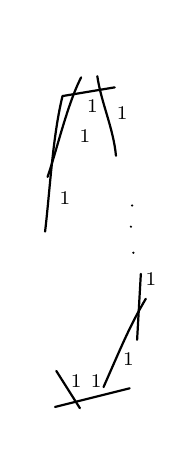
\begin{tikzpicture}[x=.0158cm,y=-.0158cm,line width=.8pt,line cap=round,line join=round,every node/.style={inner sep=0pt,font=\scriptsize}]
\path[use as bounding box] (0,0) rectangle (112,318);
\draw (14,164) .. controls (18,130) and (20,88) .. (28,55);
\draw (16,120) .. controls (23,100) and (32,61) .. (43,40);
\draw (28,55) -- (70,48);
\draw (56,39) .. controls (59,60) and (69,81) .. (71,103);
\draw (91,198) -- (88,251);
\draw (61,289) .. controls (76,255) and (82,240) .. (95,218);
\draw (22,305) -- (82,290);
\draw (23,276) -- (42,306);
\node at (30,137) {$1$};
\node at (46,87) {$1$};
\node at (52,63) {$1$};
\node at (76,69) {$1$};
\node at (99,202) {$1$};
\node at (81,267) {$1$};
\node at (55,284) {$1$};
\node at (39,284) {$1$};
\fill (84,143) circle[radius=.45pt];
\fill (83,160) circle[radius=.45pt];
\fill (85,181) circle[radius=.45pt];
\end{tikzpicture}}} &
\parbox[c][5.45cm][c]{1.82cm}{\figure{%
\begin{tikzpicture}[x=.0158cm,y=-.0158cm,line width=.8pt,line cap=round,line join=round,every node/.style={inner sep=0pt,font=\scriptsize}]
\path[use as bounding box] (0,0) rectangle (112,318);
\draw (30,70) .. controls (48,107) and (51,128) .. (53,170) .. controls (52,133) and (53,110) .. (74,69);
\node at (78,90) {$1$};
\end{tikzpicture}}} &
\parbox[c][5.45cm][c]{1.82cm}{\figure{%
\begin{tikzpicture}[x=.0158cm,y=-.0158cm,line width=.8pt,line cap=round,line join=round,every node/.style={inner sep=0pt,font=\scriptsize}]
\path[use as bounding box] (0,0) rectangle (112,318);
\draw (31,76) .. controls (46,108) and (53,124) .. (53,140) -- (53,183) .. controls (53,203) and (43,220) .. (32,235);
\draw (71,76) .. controls (58,110) and (53,125) .. (53,140) -- (53,183) .. controls (53,204) and (60,226) .. (75,241);
\node at (28,99) {$1$};
\node at (78,93) {$1$};
\end{tikzpicture}}} &
\parbox[c][5.45cm][c]{1.82cm}{\figure{%
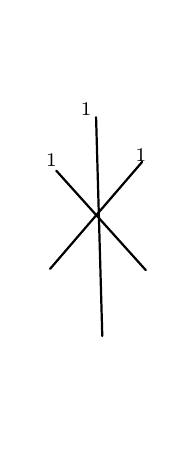
\begin{tikzpicture}[x=.0158cm,y=-.0158cm,line width=.8pt,line cap=round,line join=round,every node/.style={inner sep=0pt,font=\scriptsize}]
\path[use as bounding box] (0,0) rectangle (112,318);
\draw (55,72) -- (60,248);
\draw (23,115) -- (95,195);
\draw (92,108) -- (18,194);
\node at (47,66) {$1$};
\node at (19,107) {$1$};
\node at (91,103) {$1$};
\end{tikzpicture}}} &
\parbox[c][5.45cm][c]{1.82cm}{\figure{%
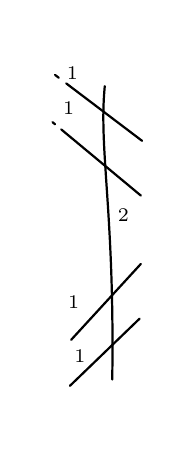
\begin{tikzpicture}[x=.0158cm,y=-.0158cm,line width=.8pt,line cap=round,line join=round,every node/.style={inner sep=0pt,font=\scriptsize}]
\path[use as bounding box] (0,0) rectangle (112,318);
\draw (62,47) .. controls (57,98) and (70,148) .. (68,283);
\draw (22,38) -- (25,40.27);
\draw (31,44.81) -- (92,91);
\draw (20,76) -- (22,77.66);
\draw (27,81.82) -- (91,135);
\draw (35,251) -- (91,190);
\draw (34,288) -- (90,234);
\node at (36,37) {$1$};
\node at (33,65) {$1$};
\node at (77,151) {$2$};
\node at (37,221) {$1$};
\node at (42,264) {$1$};
\end{tikzpicture}}} &
\parbox[c][5.45cm][c]{1.82cm}{\figure{%
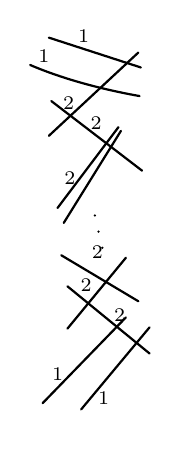
\begin{tikzpicture}[x=.0158cm,y=-.0158cm,line width=.8pt,line cap=round,line join=round,every node/.style={inner sep=0pt,font=\scriptsize}]
\path[use as bounding box] (0,0) rectangle (112,318);
\draw (17,8) -- (91,32);
\draw (2,30) .. controls (30,42) and (62,50) .. (90,55);
\draw (17,87) -- (89,20);
\draw (19,59) -- (92,115);
\draw (24,145) -- (73,80);
\draw (29,157) -- (75,83);
\draw (27,183) -- (89,220);
\draw (32,208) -- (98,262);
\draw (32,242) -- (79,185);
\draw (12,302) -- (79,233);
\draw (43,307) -- (98,241);
\node at (45,7) {$1$};
\node at (13,23) {$1$};
\node at (33,61) {$2$};
\node at (55,77) {$2$};
\node at (34,121) {$2$};
\node at (56,181) {$2$};
\node at (47,207) {$2$};
\node at (74,231) {$2$};
\node at (24,279) {$1$};
\node at (61,298) {$1$};
\fill (54,151) circle[radius=.45pt];
\fill (57,164) circle[radius=.45pt];
\fill (60,177) circle[radius=.45pt];
\end{tikzpicture}}} &
\parbox[c][5.45cm][c]{1.82cm}{\figure{%
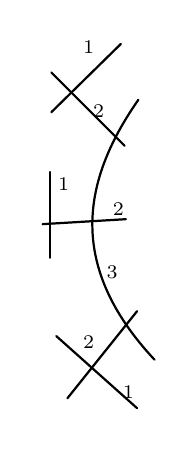
\begin{tikzpicture}[x=.0158cm,y=-.0158cm,line width=.8pt,line cap=round,line join=round,every node/.style={inner sep=0pt,font=\scriptsize}]
\path[use as bounding box] (0,0) rectangle (112,318);
\draw (19,68) -- (75,13);
\draw (19,36) -- (78,95);
\draw (89,58) .. controls (43,124) and (32,192) .. (102,267);
\draw (18,116) -- (18,185);
\draw (12,158) -- (79,154);
\draw (32,298) -- (88,228);
\draw (23,248) -- (88,306);
\node at (49,16) {$1$};
\node at (57,67) {$2$};
\node at (29,126) {$1$};
\node at (73,146) {$2$};
\node at (68,197) {$3$};
\node at (49,253) {$2$};
\node at (81,293) {$1$};
\end{tikzpicture}}} &
\parbox[c][5.45cm][c]{1.82cm}{\figure{%
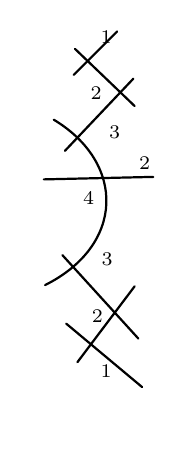
\begin{tikzpicture}[x=.0158cm,y=-.0158cm,line width=.8pt,line cap=round,line join=round,every node/.style={inner sep=0pt,font=\scriptsize}]
\path[use as bounding box] (0,0) rectangle (112,318);
\draw (37,38) -- (72,3);
\draw (38,17) -- (86,63);
\draw (30,99) -- (85,41);
\draw (21,74) .. controls (79,109) and (78,175) .. (14,207);
\draw (13,122) -- (101,120);
\draw (28,183) -- (89,250);
\draw (40,269) -- (86,208);
\draw (31,238) -- (92,289);
\node at (63,8) {$1$};
\node at (55,53) {$2$};
\node at (70,84) {$3$};
\node at (94,109) {$2$};
\node at (49,137) {$4$};
\node at (64,186) {$3$};
\node at (56,232) {$2$};
\node at (63,276) {$1$};
\end{tikzpicture}}} &
\parbox[c][5.45cm][c]{1.82cm}{\figure{%
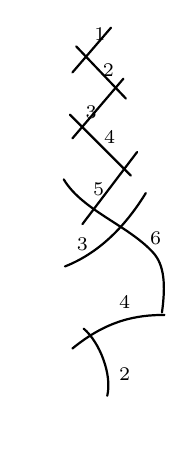
\begin{tikzpicture}[x=.0158cm,y=-.0158cm,line width=.8pt,line cap=round,line join=round,every node/.style={inner sep=0pt,font=\scriptsize}]
\path[use as bounding box] (0,0) rectangle (112,318);
\draw (36,36) -- (67,0);
\draw (39,15) -- (79,57);
\draw (36,89) -- (77,41);
\draw (34,70) -- (83,119);
\draw (44,158) -- (88,100);
\draw (29,122) .. controls (44,147) and (81,159) .. (101,181) .. controls (110,191) and (111,207) .. (108,229);
\draw (30,192) .. controls (58,181) and (79,159) .. (95,133);
\draw (36,258) .. controls (64,235) and (88,231) .. (110,231);
\draw (45,242) .. controls (58,253) and (68,279) .. (64,296);
\node at (58,5) {$\unsure{1}$};
\node at (65,34) {$2$};
\node at (51,68) {$3$};
\node at (66,88) {$4$};
\node at (57,130) {$5$};
\node at (44,174) {$3$};
\node at (103,169) {$6$};
\node at (78,221) {$4$};
\node at (78,279) {$2$};
\end{tikzpicture}}} \\ \hline
\shortstack[l]{$\deleted{\unsure{m|n}}=\,$number of\\irred. components} &
1 & \nu & 1 & 2 & 3 & 5 & 5+\nu & 7 & 8 & 9 \\ \hline
\shortstack[l]{type of group $E(K)/E_0(K)$\\$\approx\widetilde X_0(k)/\widetilde E_0(k)$} &
(1)&(\nu)&(1)&(2)&(3)&(2\times2)&
\substack{(4),\,\nu\ \text{odd}\\2\times2),\,\nu\ \text{even}}&
(3)&(2)&(1)\\ \hline
\widetilde E_0(k)\simeq E_0(K)/E_1(K) &
\widetilde E(k)&k^{*}&k^{+}&k^{+}&k^{+}&k^{+}&k^{+}&k^{+}&k^{+}&k^{+}\\ \hline
\multicolumn{11}{|l|}{\text{S\quad S\quad BELOW THIS LINE THINGS ARE VALID ONLY FOR }\operatorname{CHAR}(k)\ne2,3\quad\text{S}}\\ \hline
v(\Delta_v)&0&\nu&2&3&4&6&6+\nu&8&9&10\\ \hline
\shortstack[l]{$v(\Delta_v)+1-m=f$\\$={}$exp. of $\mathfrak p$ in cond.}&
0&1&2&2&2&2&2&2&2&2\\ \hline
\text{behavior of }j&
v(j)\geq0&
\substack{\deleted{\unsure{v(j)|j}}\\v(j)=-\nu}&
\widetilde j=0&\widetilde j=1728&\widetilde j=0&
v(j)\geq0&v(j)=-\nu&\widetilde j=0&\widetilde j=1728&\widetilde j=0\\ \hline
\end{array}$}}

Here $\widetilde X_0$ denotes the non-singular part of the fiber. This is a (non-connected in general) algebraic group over $k$, whose connected component is $\widetilde E_0$. We have $E(K)/E_1(K)\approx\widetilde X_0(k)$, the isom induced by the reduction map, and assuming now $R$ complete. Note that if $p=\operatorname{char} k\ne2,3$, then we have minimality $\Longleftrightarrow$ \uline{either} $v(\Delta)<12$, \uline{or} $v(\Delta)+v(j)<12$. Also, if $p\ne2,3$, and $f=2$, then $E_0(K)$ is uniquely divisible by $2$ and $3$, while $E(K)/E_0(K)$ is killed by $12$, Hence $E(K)/E_0(K)$ is isomorphic to the group of points in $E(K)$ which are killed by $12$ in \unsure{this}%
\unsure{'|{}}
% archive sheet number: 9
\clearpage
